\documentclass{beamer}


\usepackage{amsmath}
\usepackage{listings}
\usepackage{color}

\definecolor{codegreen}{rgb}{0,0.6,0}

\lstset{ %
  basicstyle=\fontsize{9}{11}\ttfamily,
  backgroundcolor=\color{white},   % choose the background color; you must add \usepackage{color} or \usepackage{xcolor}; should come as last argument
  breakatwhitespace=false,         % sets if automatic breaks should only happen at whitespace
  captionpos=b,                    % sets the caption-position to bottom
  commentstyle=\color{codegreen},    % comment style
  keepspaces=true,                 % keeps spaces in text, useful for keeping indentation of code (possibly needs columns=flexible)
  rulecolor=\color{black},         % if not set, the frame-color may be changed on line-breaks within not-black text (e.g. comments (green here))
  showspaces=false,                % show spaces everywhere adding particular underscores; it overrides 'showstringspaces'
  showstringspaces=false,          % underline spaces within strings only
  showtabs=false,                  % show tabs within strings adding particular underscores
  tabsize=2,	                     % sets default tabsize to 2 spaces
}





\mode<presentation> {

% The Beamer class comes with a number of default slide themes
% which change the colors and layouts of slides. Below this is a list
% of all the themes, uncomment each in turn to see what they look like.

%\usetheme{default}
%\usetheme{AnnArbor}
%\usetheme{Antibes}
%\usetheme{Bergen}
%\usetheme{Berkeley}
%\usetheme{Berlin}
%\usetheme{Boadilla}
%\usetheme{CambridgeUS}
%\usetheme{Copenhagen}
%\usetheme{Darmstadt}
%\usetheme{Dresden}
%\usetheme{Frankfurt}
%\usetheme{Goettingen}
%\usetheme{Hannover}
%\usetheme{Ilmenau}
%\usetheme{JuanLesPins}
%\usetheme{Luebeck}
\usetheme{Madrid}
%\usetheme{Malmoe}
%\usetheme{Marburg}
%\usetheme{Montpellier}
%\usetheme{PaloAlto}
%\usetheme{Pittsburgh}
%\usetheme{Rochester}
%\usetheme{Singapore}
%\usetheme{Szeged}
%\usetheme{Warsaw}

% As well as themes, the Beamer class has a number of color themes
% for any slide theme. Uncomment each of these in turn to see how it
% changes the colors of your current slide theme.

%\usecolortheme{albatross}
%\usecolortheme{beaver}
%\usecolortheme{beetle}
%\usecolortheme{crane}
%\usecolortheme{dolphin}
%\usecolortheme{dove}
%\usecolortheme{fly}
%\usecolortheme{lily}
%\usecolortheme{orchid}
%\usecolortheme{rose}
%\usecolortheme{seagull}
%\usecolortheme{seahorse}
%\usecolortheme{whale}
%\usecolortheme{wolverine}

%\setbeamertemplate{footline} % To remove the footer line in all slides uncomment this line
%\setbeamertemplate{footline}[page number] % To replace the footer line in all slides with a simple slide count uncomment this line

%\setbeamertemplate{navigation symbols}{} % To remove the navigation symbols from the bottom of all slides uncomment this line
}

\usepackage{graphicx} % Allows including images
\usepackage{booktabs} % Allows the use of \toprule, \midrule and \bottomrule in tables

%----------------------------------------------------------------------------------------
%	TITLE PAGE
%----------------------------------------------------------------------------------------

\title[Short title]{
Emulate the \texttt{persp()} plot and \texttt{filled.contour()} plot on \textbf{gridGraphics}
} % The short title appears at the bottom of every slide, the full title is only on the title page

\author{Zhijian Wen} % Your name
\institute[UOA] % Your institution as it will appear on the bottom of every slide, may be shorthand to save space
{
University of Auckland \\ % Your institution for the title page
\medskip
\textit{jwen246@aucklanduni.ac.nz} % Your email address
}
\date{\today} % Date, can be changed to a custom date

\usepackage{Sweave}
\begin{document}
\Sconcordance{concordance:presentation.tex:presentation.Rnw:%
1 106 1 1 0 49 1 1 7 2 0 2 1 3 0 1 2 10 1 1 22 1 0 1 1 3 0 1 2 9 1 1 2 %
1 0 1 1 3 0 1 2 29 1 1 8 151 1 1 12 202 1 1 41 66 1 1 88 76 1}


\begin{frame}
\titlepage % Print the title page as the first slide
\end{frame}


%----------------------------------------------------------------------------------------
%	PRESENTATION SLIDES
%----------------------------------------------------------------------------------------

%------------------------------------------------

\begin{frame}[fragile]
\begin{center}
  \Huge Introduction
\end{center}
\end{frame}

%------------------------------------------------

\begin{frame}[fragile]

\frametitle{Introduction}
What is \textbf{graphics} and what is \textbf{grid} ?
\begin{center}
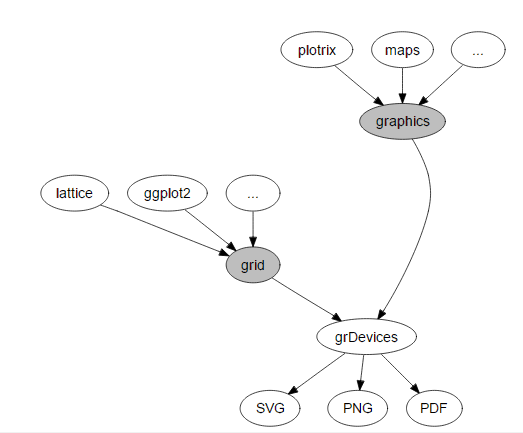
\includegraphics[width = 8cm, height = 6cm]{plot/grid_and_graphics.PNG}
\end{center}

\end{frame}

%------------------------------------------------

\begin{frame}[fragile]
\frametitle{Introduction}
Then, what is \textbf{gridGraphics}? \\

\begin{enumerate}
	\item A \textbf{R} package 
	\item A ``translator'' that translates a \textbf{graphics}-plot to a \textbf{grid}-plot 
	\item With a main function \texttt{grid.echo()}.
\end{enumerate}

\end{frame}



%------------------------------------------------

\begin{frame}[fragile]

\frametitle{Introduction}

What is \textbf{gridGraphics}?
\begin{center}
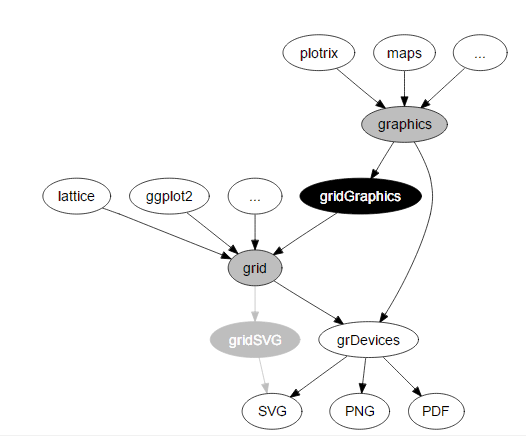
\includegraphics[width = 8cm, height = 6cm]{plot/grid_graphics.png}
\end{center}

\end{frame}

%------------------------------------------------

\begin{frame}[fragile]
\frametitle{Example}
\begin{Schunk}
\begin{Sinput}
> plot(cars$dist ~ cars$speed, pch = 16, 
+      col = 'orange', main = 'Distance vs Speed')
> library(gridGraphics)
> grid.echo()
\end{Sinput}
\end{Schunk}

\begin{center}
  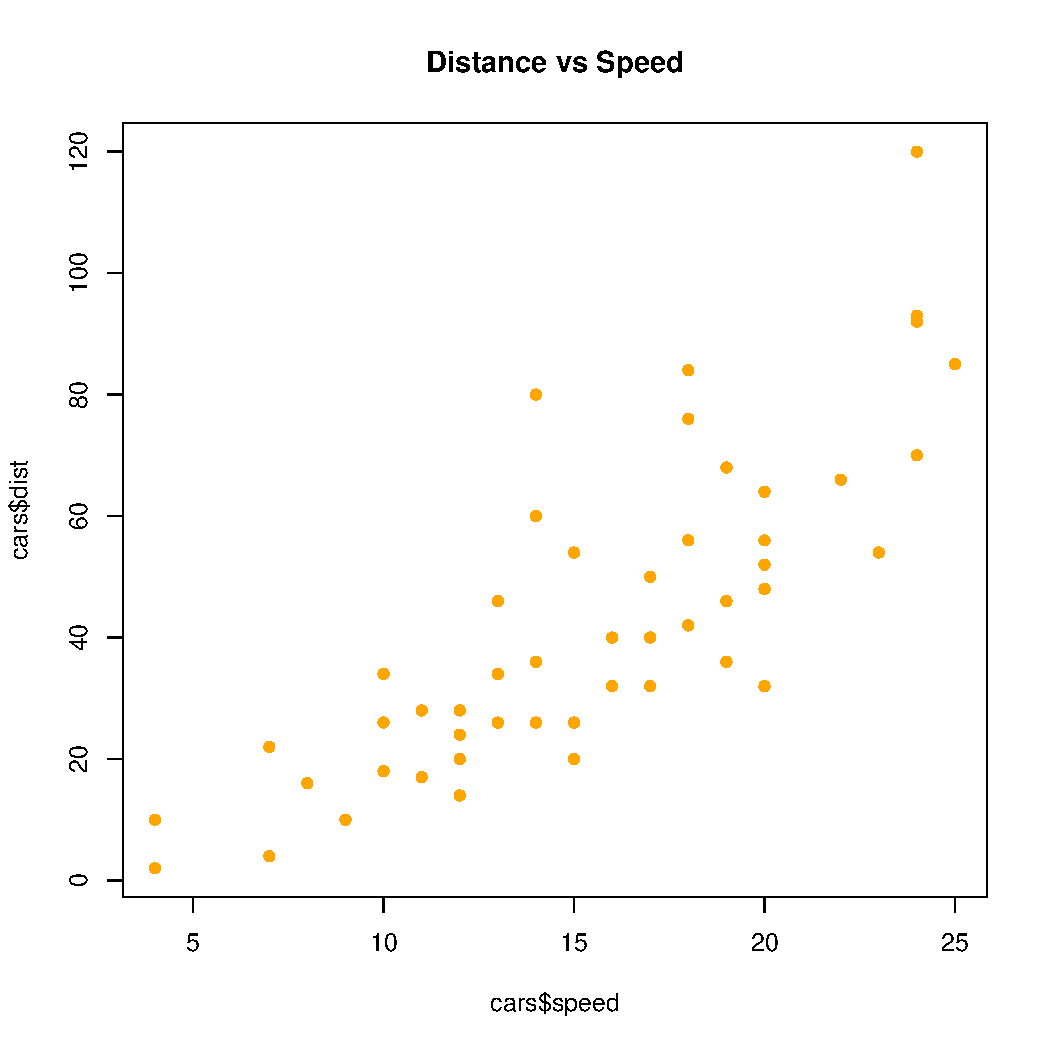
\includegraphics[height = 5.5cm, width = 5.5cm]{plot/intro_1.pdf}
  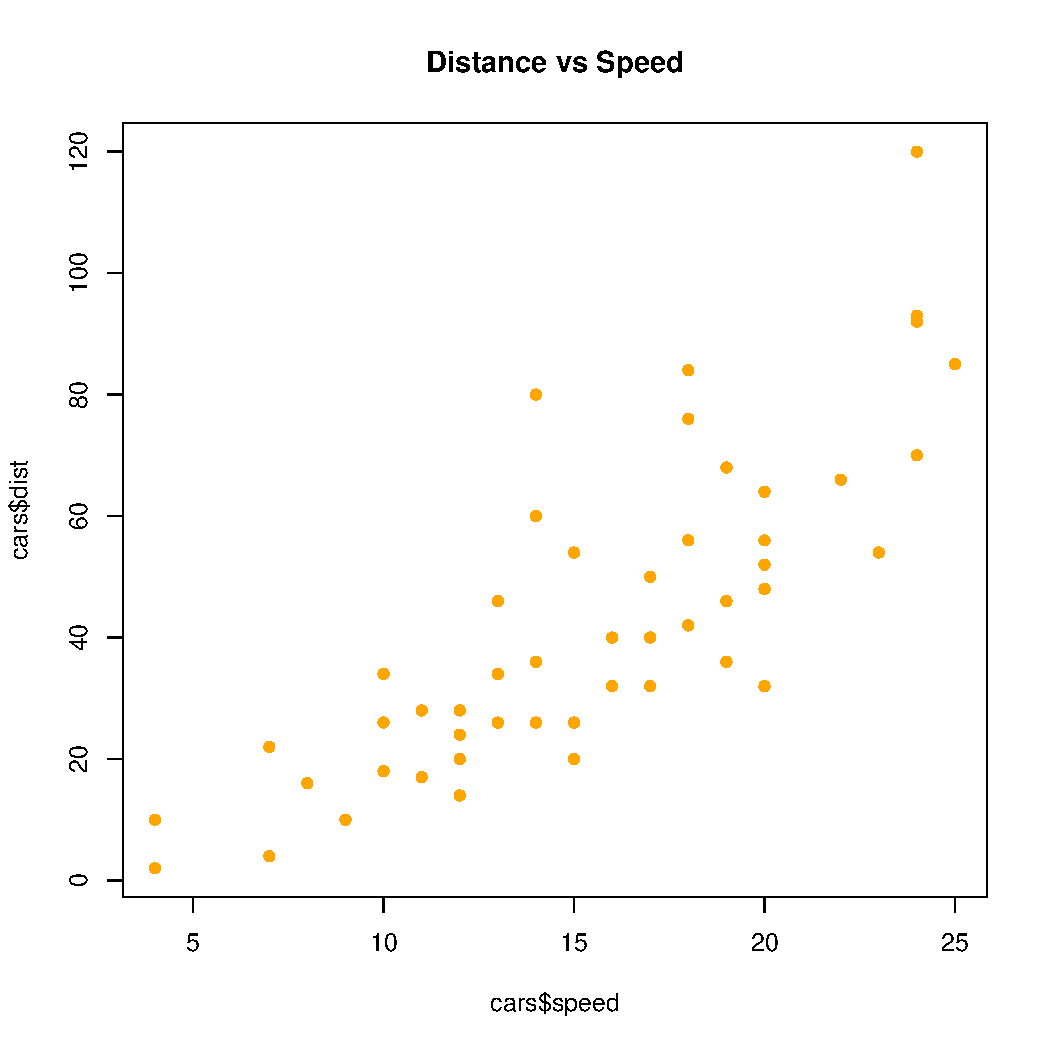
\includegraphics[height = 5.5cm, width = 5.5cm]{plot/intro_2.pdf}
\end{center}
\end{frame}

%------------------------------------------------

\begin{frame}[fragile]
\frametitle{The problem}
\begin{Schunk}
\begin{Sinput}
> Persian_Rug_Art() ##filled.contour()
> grid.echo()
\end{Sinput}
\end{Schunk}
\begin{center}
  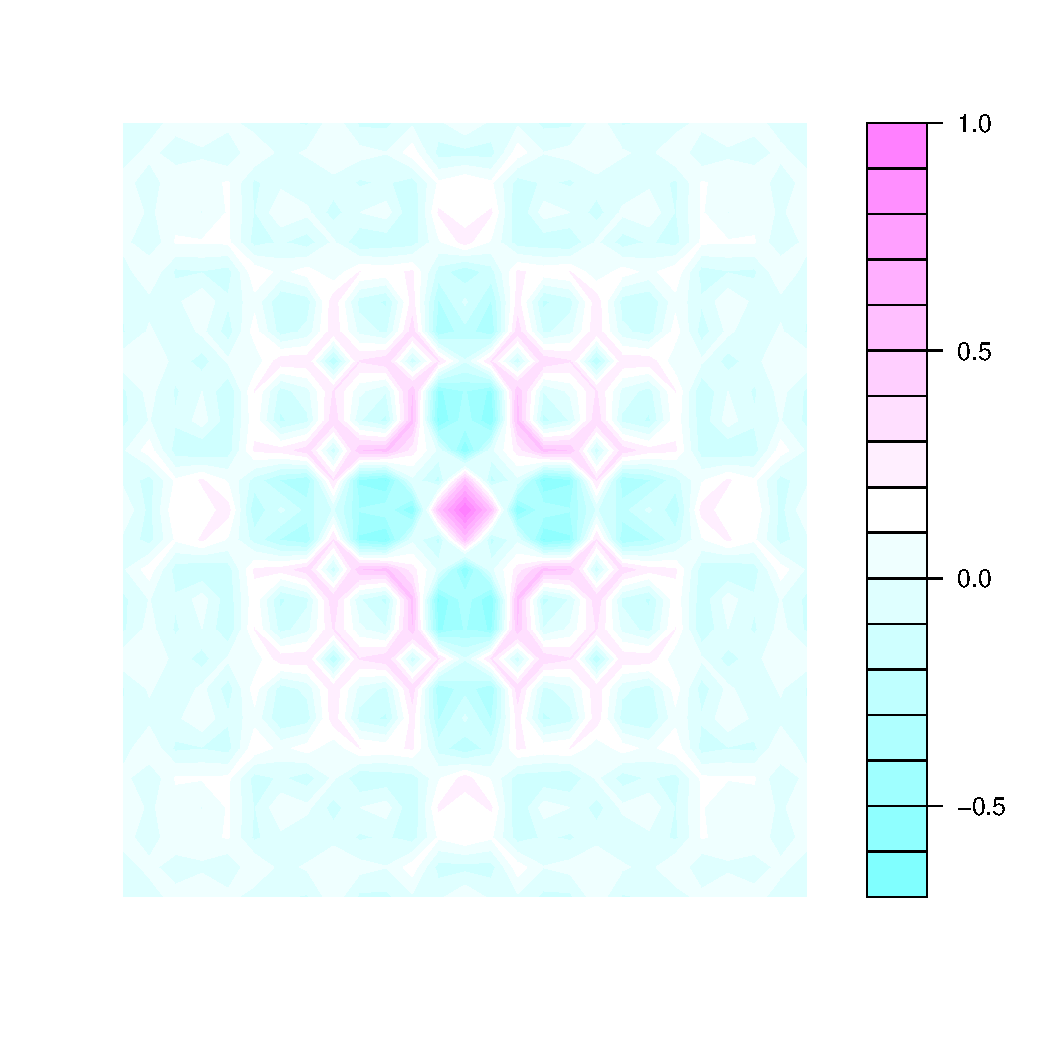
\includegraphics[height = 5.5cm, width = 5.5cm]{plot/report_fill_1}
  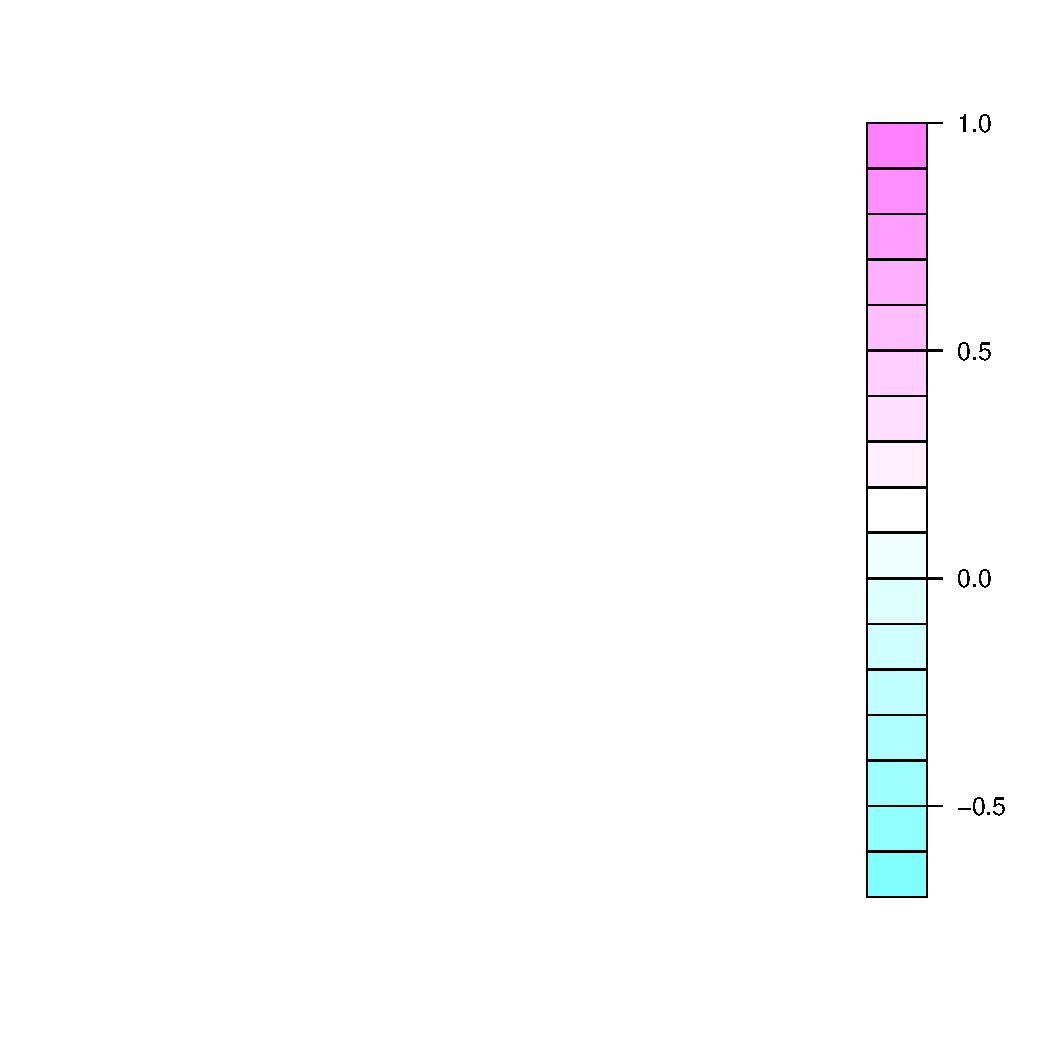
\includegraphics[height = 5.5cm, width = 5.5cm]{plot/report_fill_2}
\end{center}

\end{frame}


\begin{frame}[fragile]
\frametitle{The problem}
\begin{Schunk}
\begin{Sinput}
> Sinc_Curve() ##persp()
> grid.echo()
\end{Sinput}
\end{Schunk}
\begin{center}
  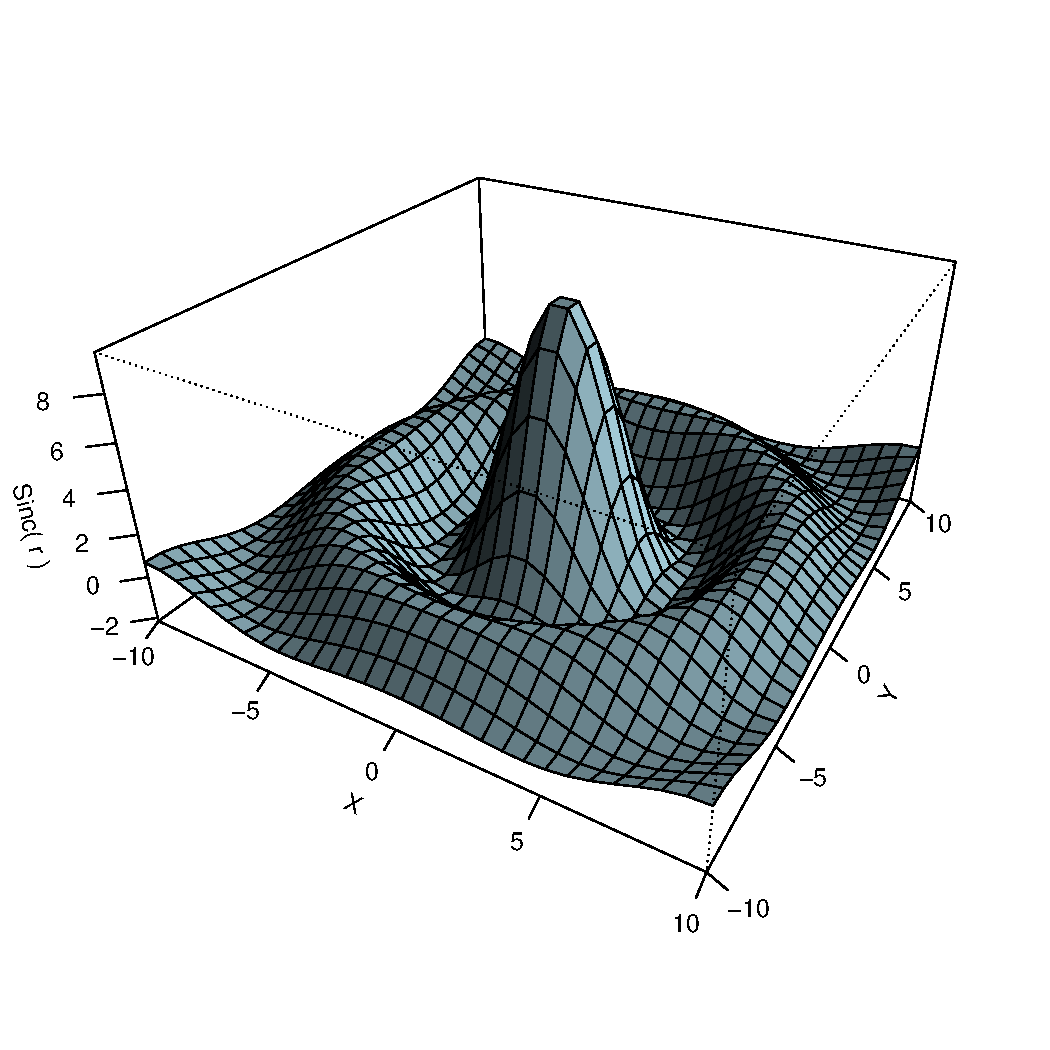
\includegraphics[height = 5.5cm, width = 5.5cm]{plot/persp_1}
  
\includegraphics[height = 5.5cm, width = 5.5cm]{plot/blank}
\end{center}
  
\end{frame}



\begin{frame}[fragile]
\begin{center}
  \Huge{The graphics engine display list}
\end{center}
\end{frame}


%------------------------------------------------

\begin{frame}[fragile]
\frametitle{The graphics engine display list}
How does \textbf{gridGraphics} works?
\begin{center}
  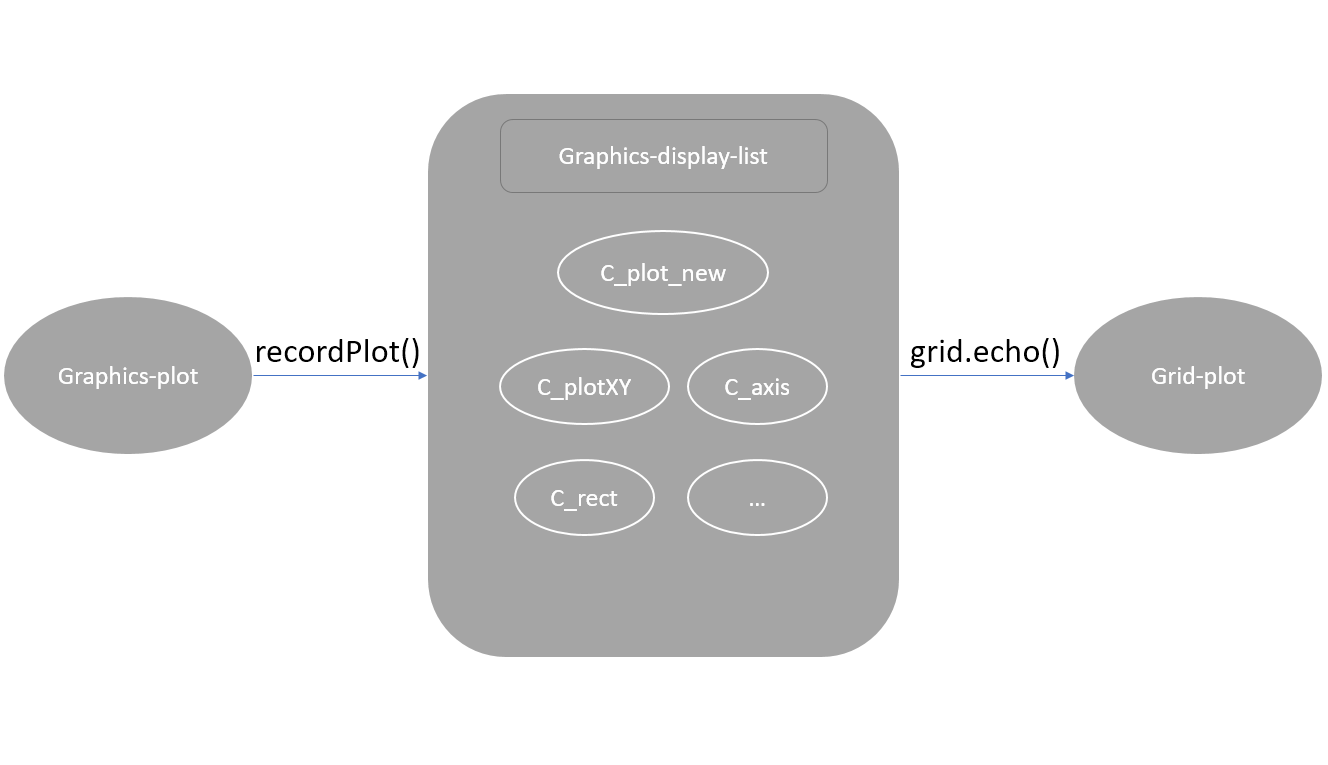
\includegraphics[height = 7.2cm, width = 12.2cm]{plot/display_list.PNG}
\end{center}
\end{frame}

%------------------------------------------------
\begin{frame}[fragile]
\frametitle{The graphics engine display list}


\begin{lstlisting}[language = R]
x <- recordPlot()
unlist(lapply(x[[1]], function(y) y[[2]][[1]]$name))
\end{lstlisting}

\begin{columns}[c]
\column{0.3\textwidth}
\begin{lstlisting}[language = R]
"C_plot_new"    
"palette2"      
"C_plot_window" 
"C_plotXY"      
"C_axis"        
"C_axis"       
"C_box"         
"C_title"    
\end{lstlisting}


\column{0.6\textwidth}
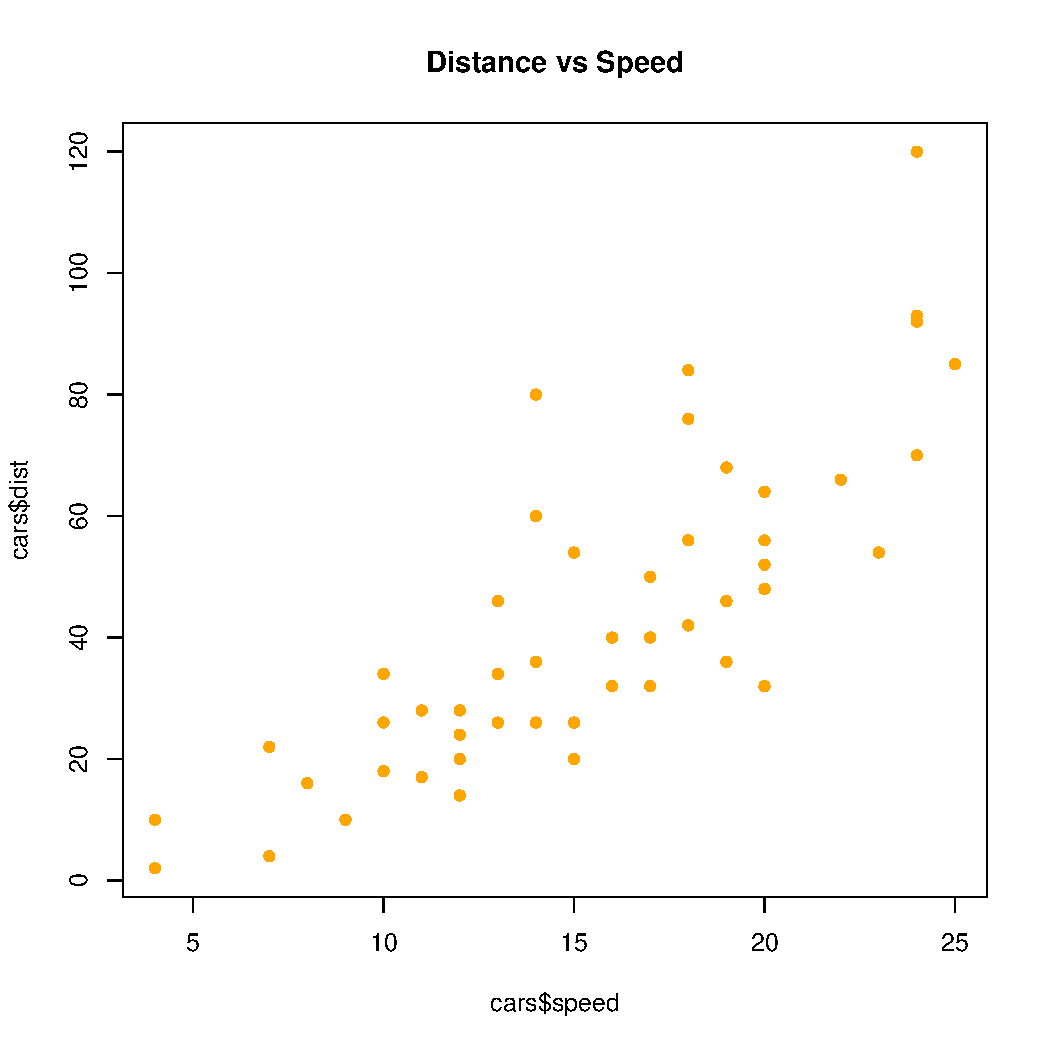
\includegraphics[height = 6cm, width = 6cm]{plot/intro_1.pdf}

\end{columns}

\end{frame}



%------------------------------------------------
\begin{frame}[fragile]
\frametitle{\texttt{C\_plot\_new} from \textbf{graphics}}

\begin{block}{The \textbf{C} code}
\begin{lstlisting}
SEXP C_plot_new(SEXP call, SEXP op, SEXP args, SEXP rho)
{
    ...
    dd = GNewPlot(GRecording(call, dd));
    ...
    GScale(0.0, 1.0, 1, dd);
    GScale(0.0, 1.0, 2, dd);
    GMapWin2Fig(dd);
    GSetState(1, dd);
    ...
}
\end{lstlisting}
\end{block}

\end{frame}


%------------------------------------------------
\begin{frame}[fragile]
\frametitle{\texttt{C\_plot\_new} from \textbf{gridGraphics}}

\begin{block}{The \textbf{R} code}
\begin{lstlisting}
C_plot_new <- function(x) {
    ...
    if (page) {
        ...
        if (get("newpage", .gridGraphicsEnv))
            grid.newpage()
        ...
        pushViewport(viewport(name=vpname("root")))
        upViewport()
        setUpInner(par)
    } else {
        setUpFigure(par)
    }
}
\end{lstlisting}
\end{block}

\end{frame}



%------------------------------------------------

\begin{frame}[fragile]
\begin{center}
\Huge Structure of the C code
\end{center}
\end{frame}


\begin{frame}[fragile]
\frametitle{Structure of the \textbf{C} code (\textif{pointers})}
\begin{block}{The problems}
\begin{lstlisting}{C}
static int LimitCheck(double *lim, double *c, double *s)
{
    if(!R_FINITE(lim[0]) || !R_FINITE(lim[1]) || 
          lim[0] >= lim[1])
    return 0;
    *s = 0.5 * fabs(lim[1] - lim[0]) ;
    *c = 0.5 * (lim[1] + lim[0]) ;
    return 1;
}
...
if(!LimitCheck(REAL(xlim), &xc, &xs))
	error(_("invalid 'x' limits"));
\end{lstlisting}
\end{block}

\end{frame}


%------------------------------------------------

\begin{frame}[fragile]
\frametitle{Structure of the \textbf{C} code (\textif{pointers})}
\begin{block}{Solution}
\begin{lstlisting}{C}
LimitCheck = function(lim){
    if(!is.finite(lim[1]) || !is.finite(lim[2]) 
            || lim[1] >= lim[2])
        stop("invalid limits");
      
    s = 0.5 * abs (lim[2] - lim[1])
    c = 0.5 * (lim[2] + lim[1])
    c(s , c)
}
xs = LimitCheck(xr)[1]
xc = LimitCheck(xr)[2]
...
\end{lstlisting}
\end{block}

\end{frame}


%------------------------------------------------

\begin{frame}[fragile]
\frametitle{How much \textbf{C} codes?}
\begin{center}

\includegraphics{plot/code.png}
\end{center}
\end{frame}



\begin{frame}[fragile]
\begin{center}
\Huge Copy or not copy?
\end{center}
\end{frame}

%------------------------------------------------

\begin{frame}[fragile]
\frametitle{Copy or not copy?}
Why just 'copy'?

\begin{enumerate}
  \item To make sure the \textbf{graphics}-plot is identical to the \textbf{grid}-plot\\~\\
\end{enumerate}

\texttt{segments(\textcolor{red}{x0 = 0}, 0.5, \textcolor{red}{x1 = 1}, 0.5, lty = 1331, lwd = 5)}
\texttt{segments(\textcolor{red}{x0 = 1}, 0.5, \textcolor{red}{x1 = 0}, 0.5, lty = 1331, lwd = 5)}
\begin{center}
  
\includegraphics[height = 2cm, width = 7cm]{plot/Rcopy.pdf}
\end{center}


Why not just 'copy'?
\begin{enumerate}
  \item Speed
\end{enumerate}


\end{frame}


%------------------------------------------------



\begin{frame}[fragile]
\frametitle{Why not just 'copy'?}

\begin{columns}[c]
\column{0.4\textwidth}
\begin{lstlisting}[language = R]
volcano_filled.contour()
xx = recordPlot()
info = xx[[1]][[12]][[2]]

dim(info[[4]])
[1] 87 61

length(info[[5]])
[1] 22
 
\end{lstlisting}
\column{0.6\textwidth}
\begin{center}
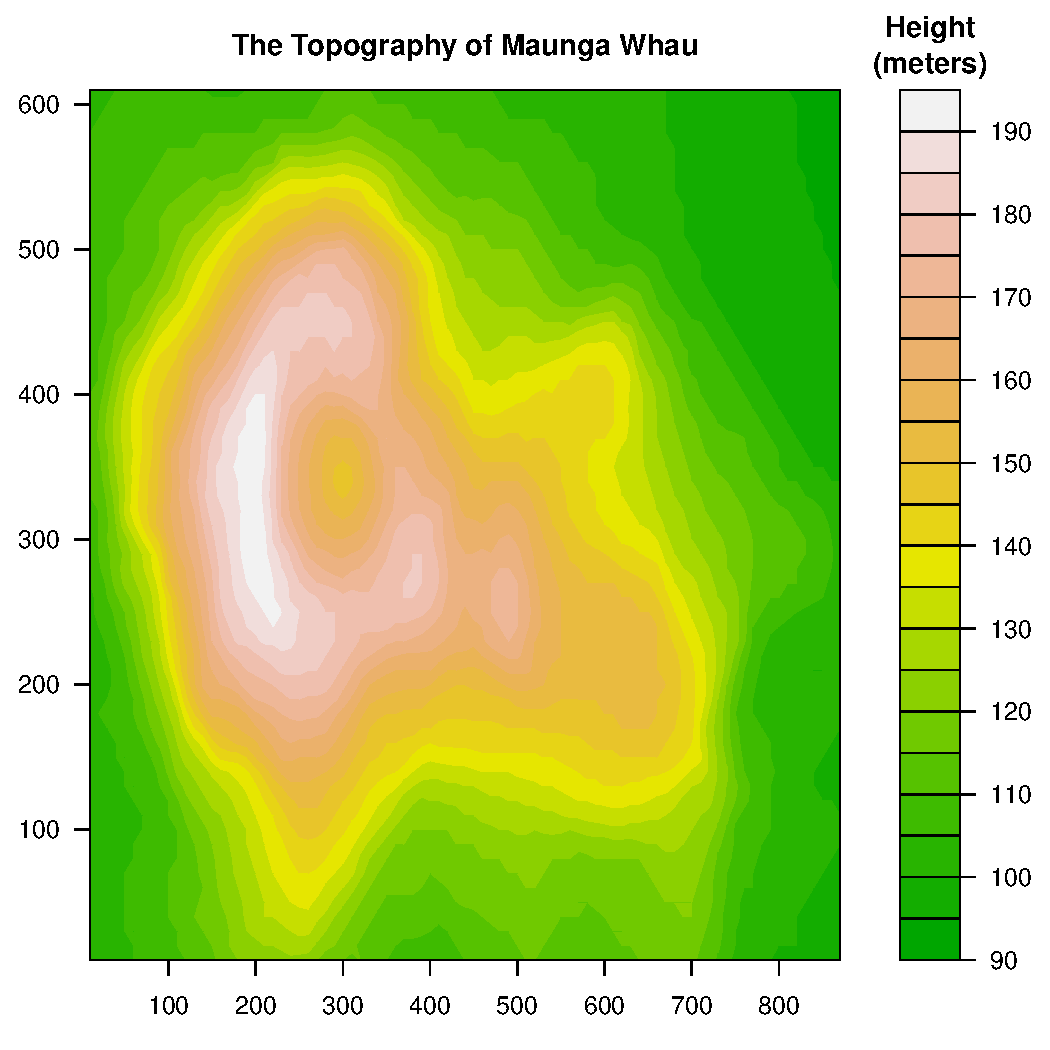
\includegraphics{plot/filled_example_1}
\end{center}

\end{columns}
There are at most (87 - 1) * (61 - 1) * (22 - 1) =  108360 polygons.


\end{frame}


%------------------------------------------------

\begin{frame}[fragile]
\frametitle{Why not just 'copy'?}

\begin{columns}[c]
\column{0.4\textwidth}
\begin{lstlisting}[language = R]
volcano_filled.contour()


## For loop 
system.time(grid.echo())

# user system elapsed
# 10.03 0.23 10.32


## vectorizetion
system.time(grid.echo())

# user system elapsed
# 1.28 0.53 1.82
\end{lstlisting}

\column{0.6\textwidth}
\begin{center}
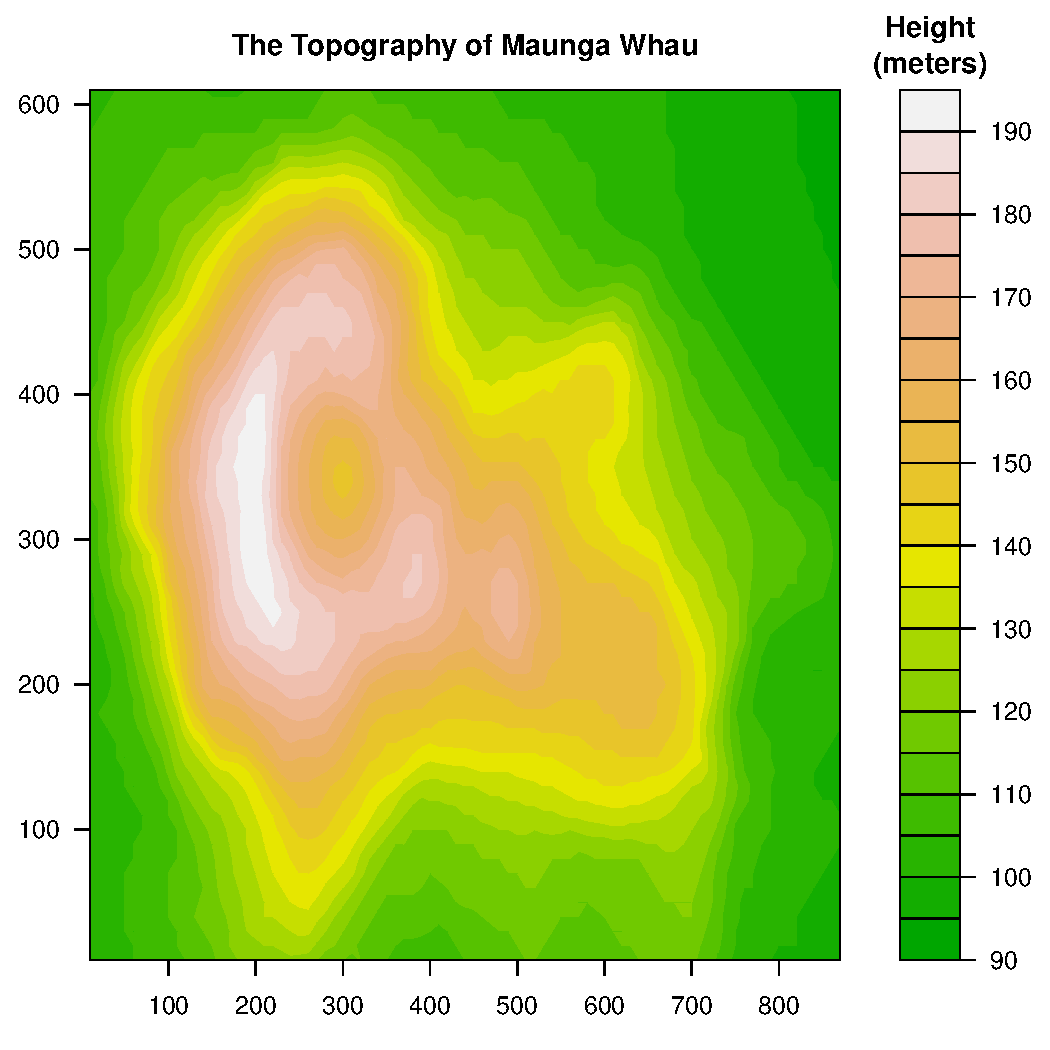
\includegraphics{plot/filled_example_1}
\end{center}

\end{columns}
\end{frame}



%------------------------------------------------
\begin{frame}[fragile]
\begin{center}
  \Huge Solution to \texttt{persp()}
\end{center}
\end{frame}


\begin{frame}[fragile]
\frametitle{Solution to \texttt{persp()}}
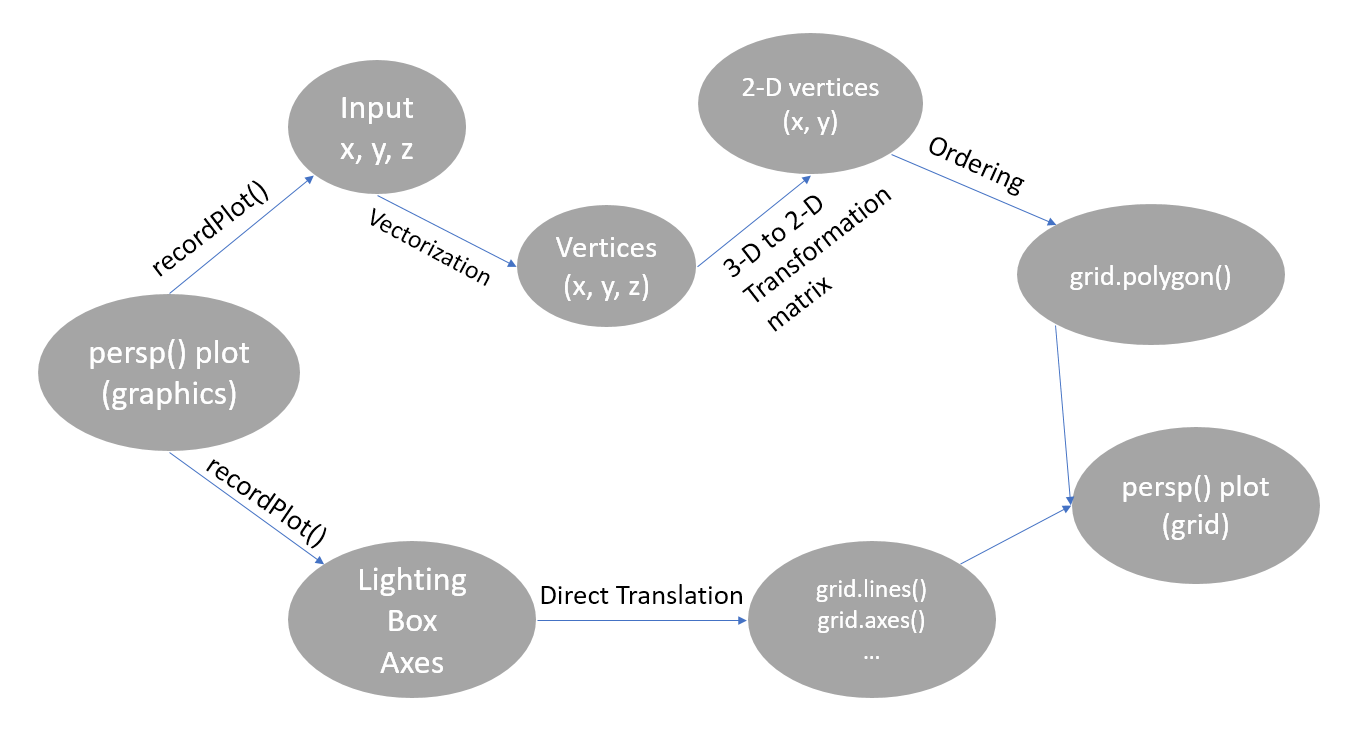
\includegraphics[height = 7cm, width = 12cm]{plot/persp_step_by_step.png}

\end{frame}



%------------------------------------------------

\begin{frame}[fragile]
\frametitle{Solution to \texttt{persp()}}

\only<1>{
  The points...
  \begin{center}
  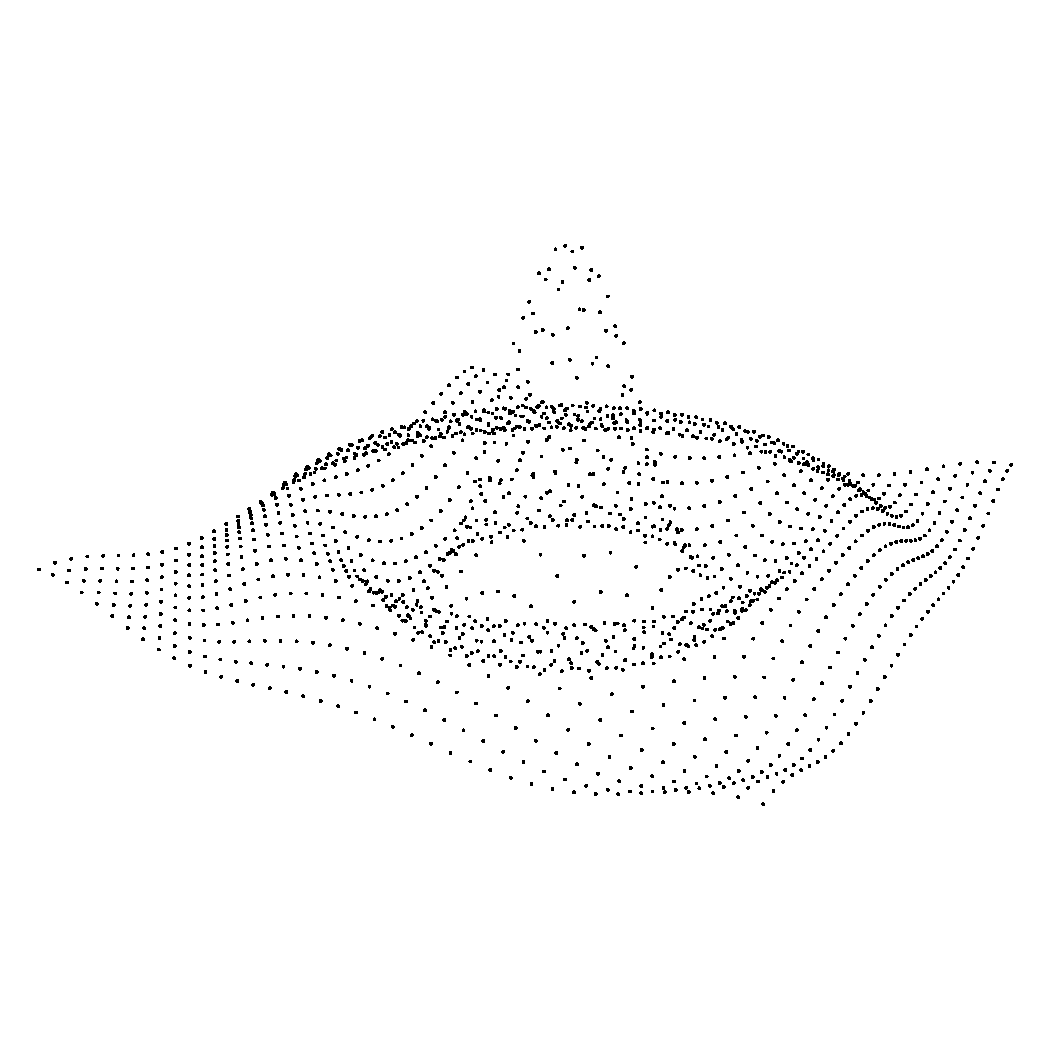
\includegraphics[height = 7cm, width = 7cm]{plot/standalone_p_1.pdf}
  \end{center}
}

\only<2>{
  The lines...
  \begin{center}
  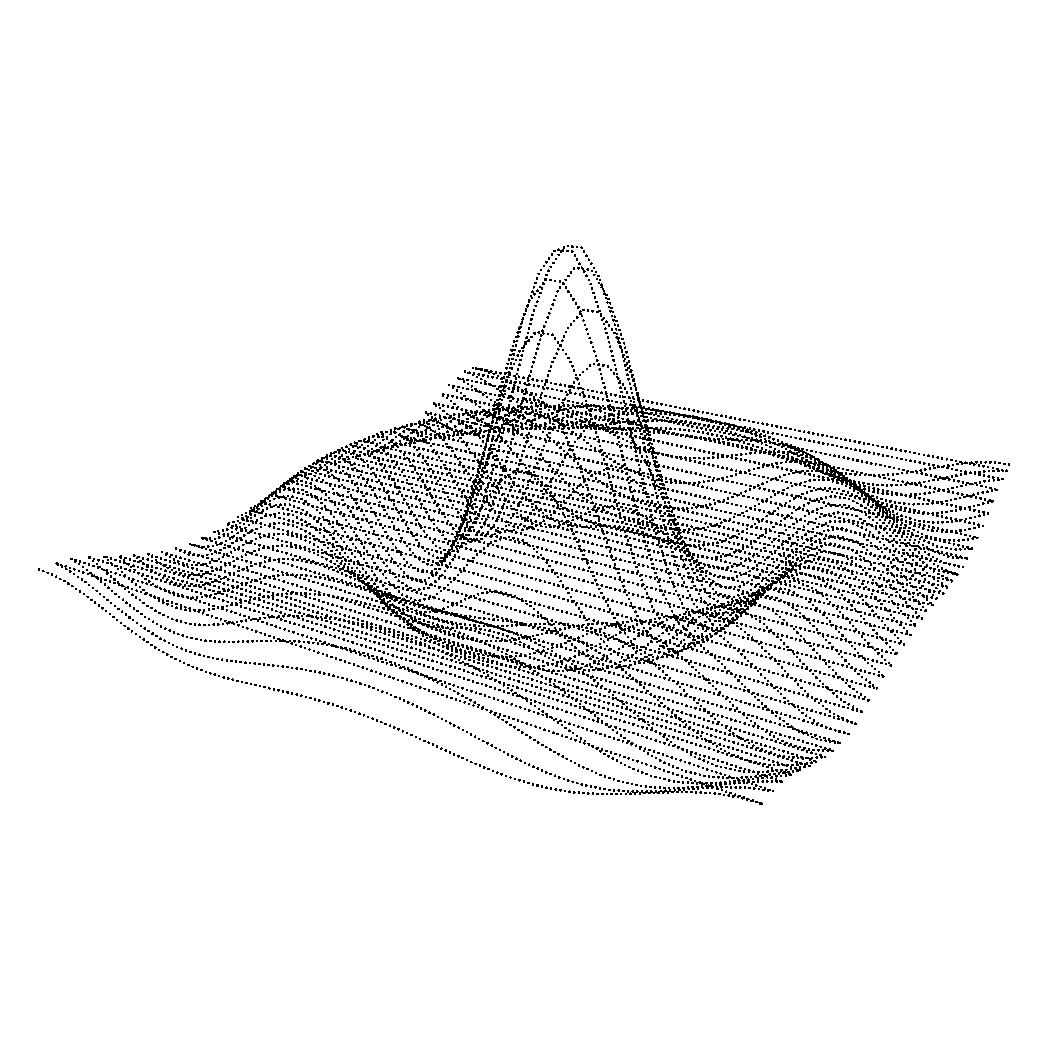
\includegraphics[height = 7cm, width = 7cm]{plot/standalone_p_2.pdf}
  \end{center}
}

\only<3>{
  The polygons(unordered)...
  \begin{center}
  
\includegraphics[height = 7cm, width = 7cm]{plot/standalone_p_3.pdf}
  \end{center}
}

\only<4>{
  And the polygons(Solution)
  \begin{center}
  
\includegraphics[height = 7cm, width = 7cm]{plot/standalone_p_4.pdf}
  \end{center}
}

\end{frame}


%------------------------------------------------
\begin{frame}
\begin{center}
\Huge Testing
\end{center}
\end{frame}


\begin{frame}[fragile]
\frametitle{Any difference?}
\begin{lstlisting}[language = R]
## left plot
Sinc_Curve(col = ??)
## right plot
Sinc_Curve(col = ??)
\end{lstlisting}

\begin{columns}[c]
\column{0.5\textwidth}
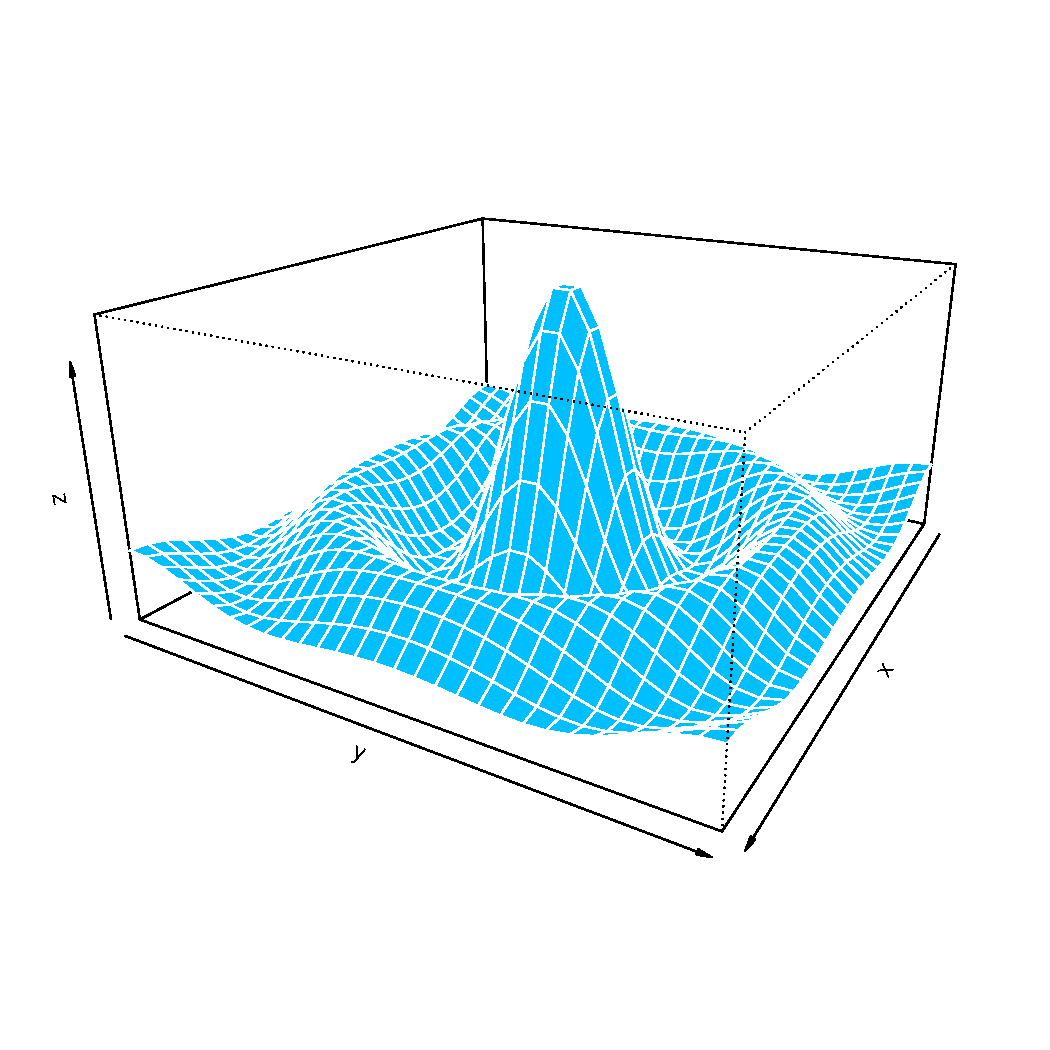
\includegraphics[height = 6cm, width = 6cm]{plot/persp_diff_1.pdf}

\column{0.5\textwidth}
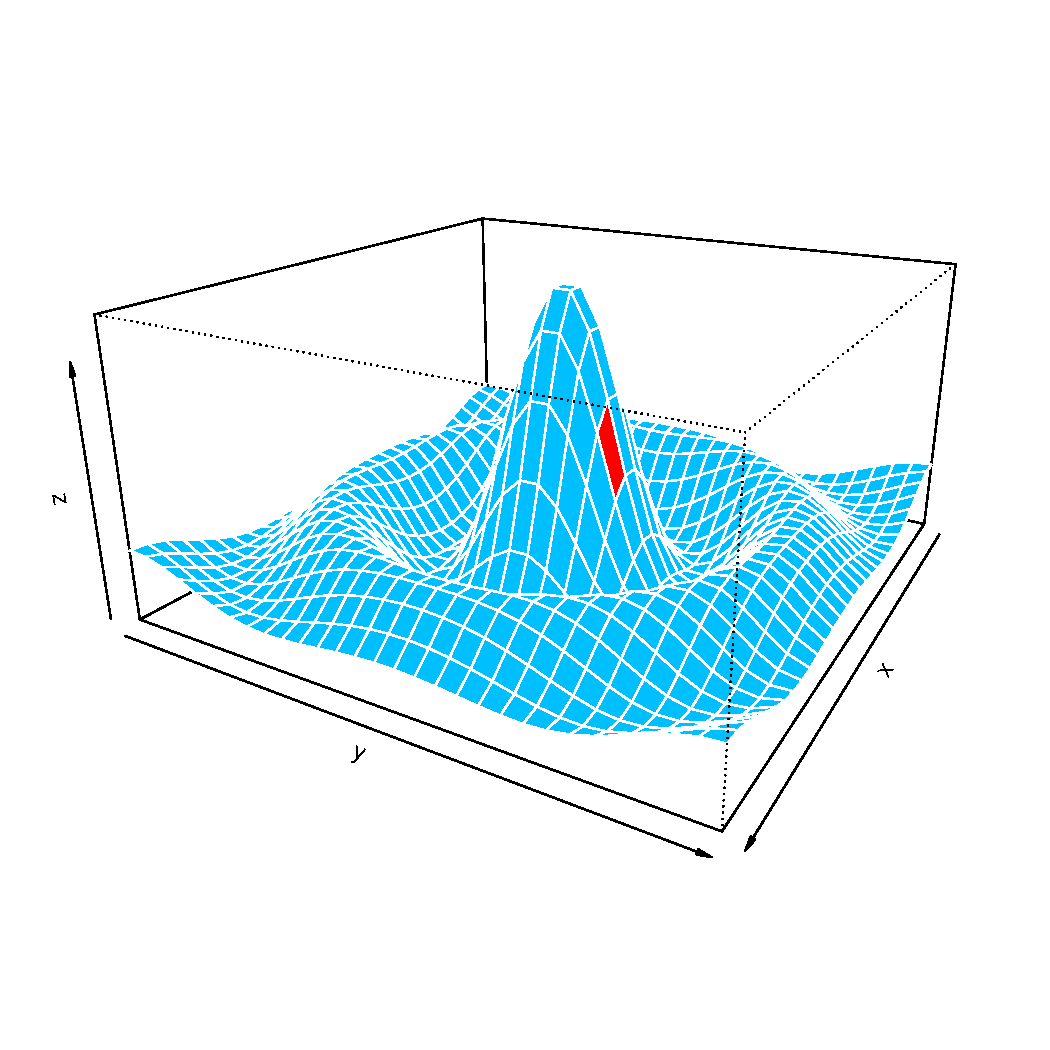
\includegraphics[height = 6cm, width = 6cm]{plot/persp_diff_2.pdf}

\end{columns}
\end{frame}



%------------------------------------------------

\begin{frame}[fragile]
\frametitle{Answers}

\begin{columns}

\column{0.5\textwidth}
\texttt{\textcolor{codegreen}{\#\# color for left plot}}\\
\texttt{col = rgb(0, \textcolor{red}{191}, 255)} \\~\\

\texttt{\textcolor{codegreen}{\#\# extra diff color for right plot}}\\
\texttt{col = rgb(0, \textcolor{red}{190}, 255)}


\column{0.5\textwidth}
\begin{center}
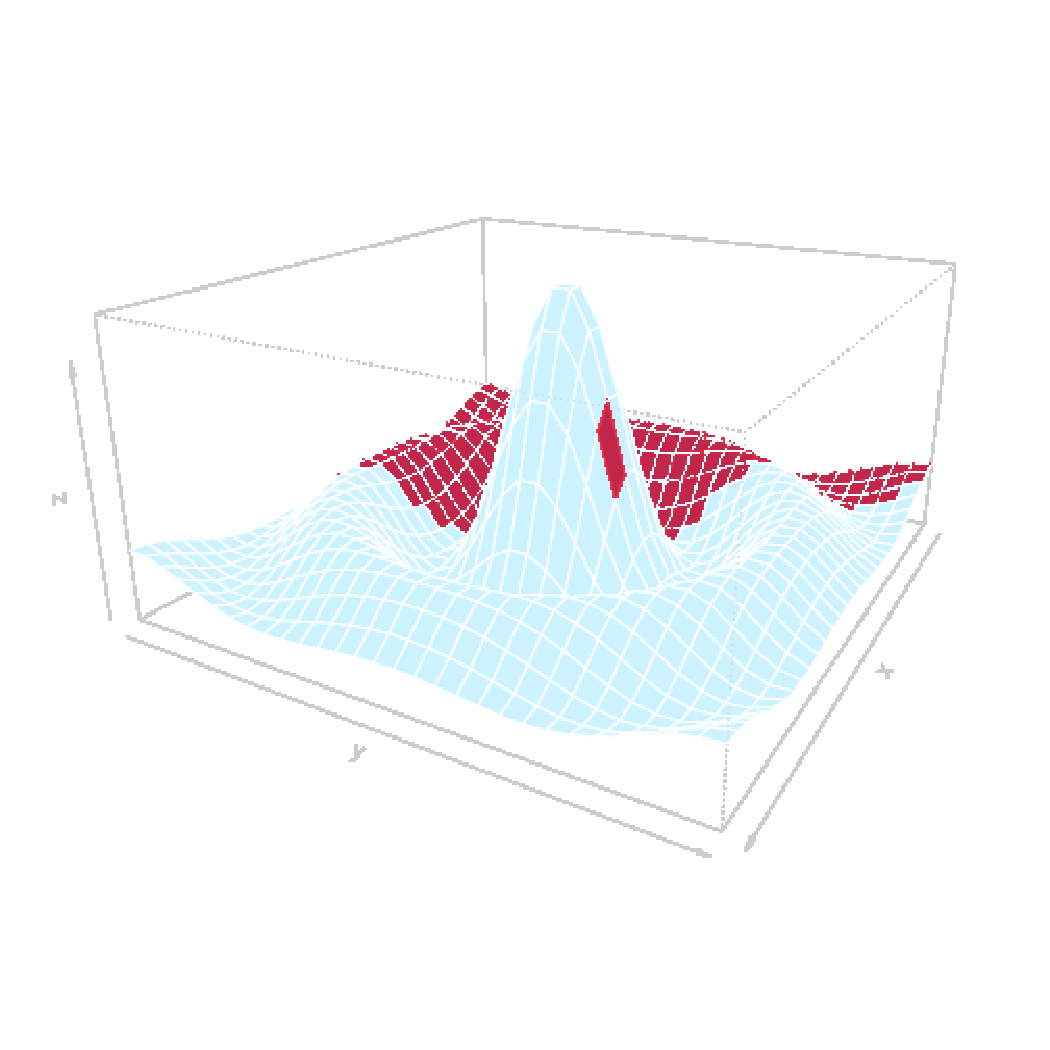
\includegraphics[height = 6cm, width = 6cm]{plot/persp_diff_3.pdf}
\end{center}

\end{columns}

\hfill \textit{*Difference dected by using the sorftware \textbf{ImageMagick}}

\end{frame}



%------------------------------------------------

\begin{frame}[fragile]
\frametitle{Final solution}

\only<1>{
  \texttt{> Torus()}\\
  \begin{center}
  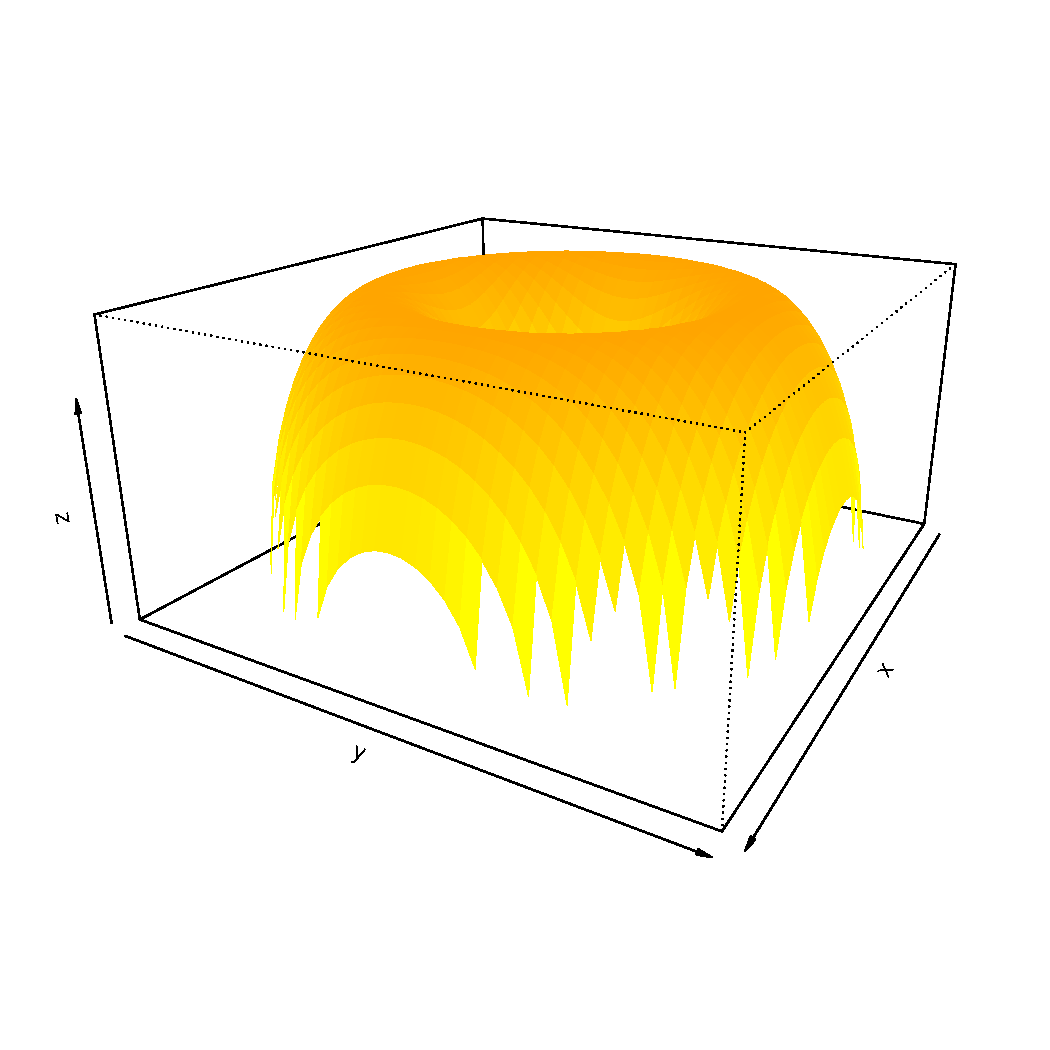
\includegraphics[height = 8cm, width = 8cm]{plot/persp_torus_1.pdf}
  \end{center}
}

\only<2>{
  \texttt{> grid.echo()} \\
  \begin{center}
  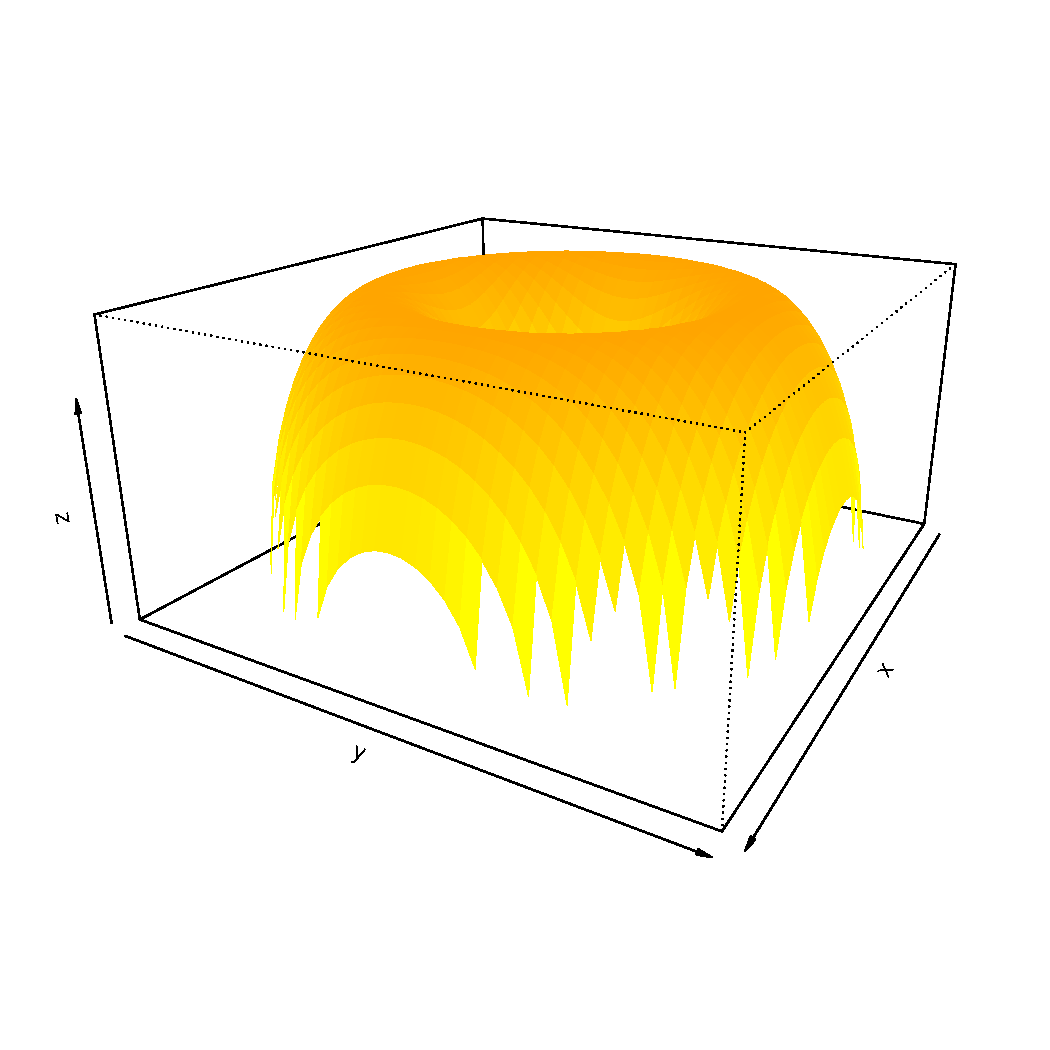
\includegraphics[height = 8cm, width = 8cm]{plot/persp_torus_2.pdf}
  \end{center}
}

\only<3>{
  Difference
  \begin{center}
  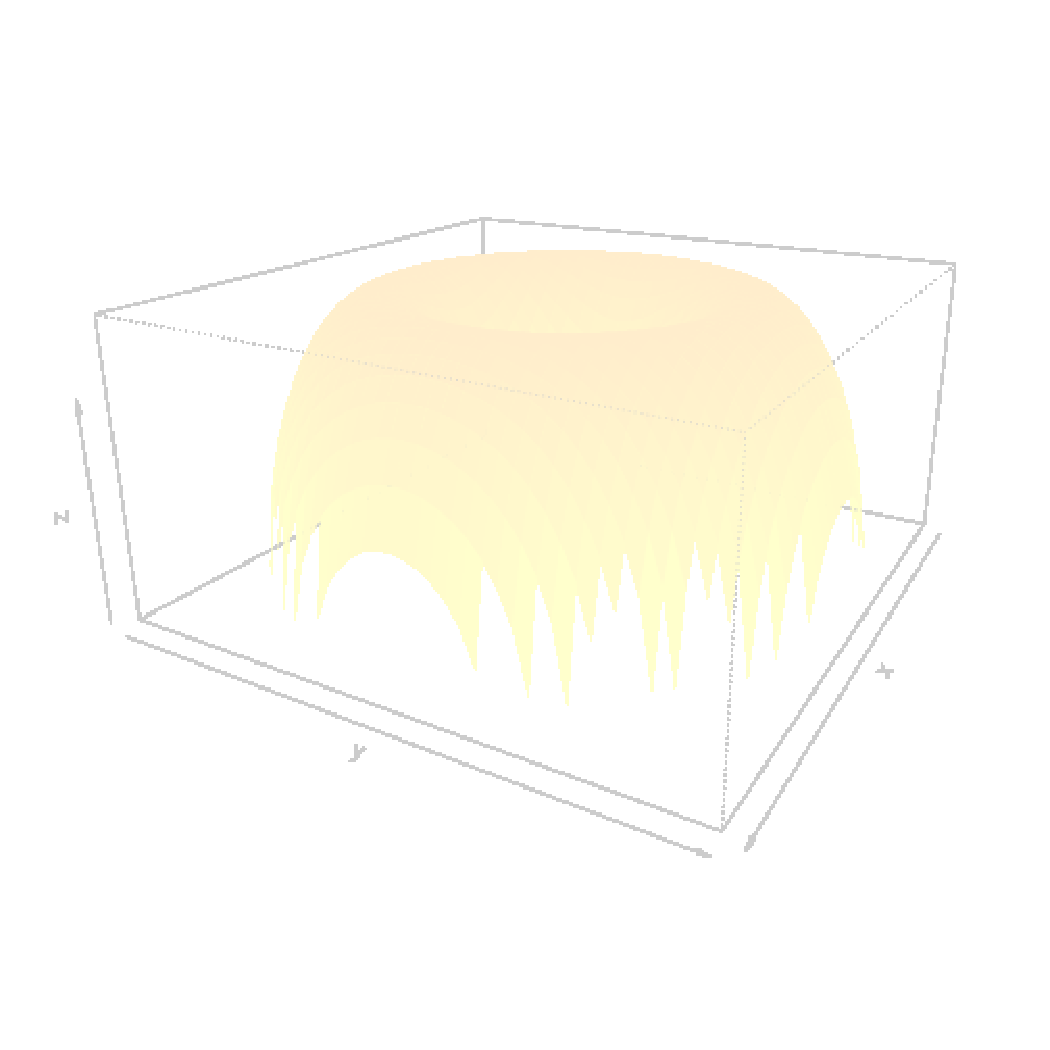
\includegraphics[height = 8cm, width = 8cm]{plot/persp_torus_diff.pdf}
  \end{center}
}


\end{frame}

%------------------------------------------------

\begin{frame}[fragile]
\frametitle{Final solution}

\only<1>{
  \texttt{> filled.contour(cos(r^2)*exp(-r/(2*pi)))}\\
  \begin{center}
  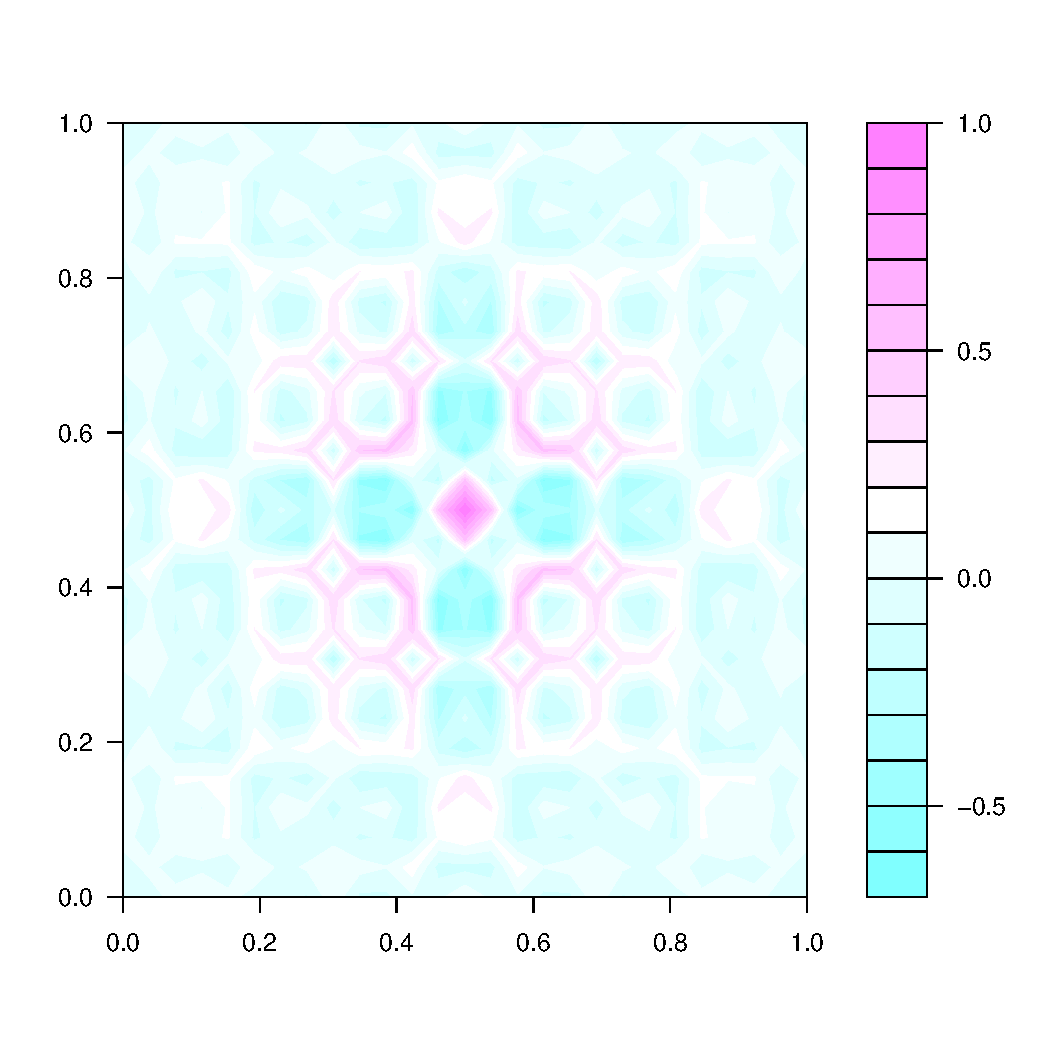
\includegraphics[height = 7cm, width = 7cm]{plot/filled_solution_1.pdf}
  \end{center}
}

\only<2>{
  \texttt{> grid.echo()} \\
  \begin{center}
  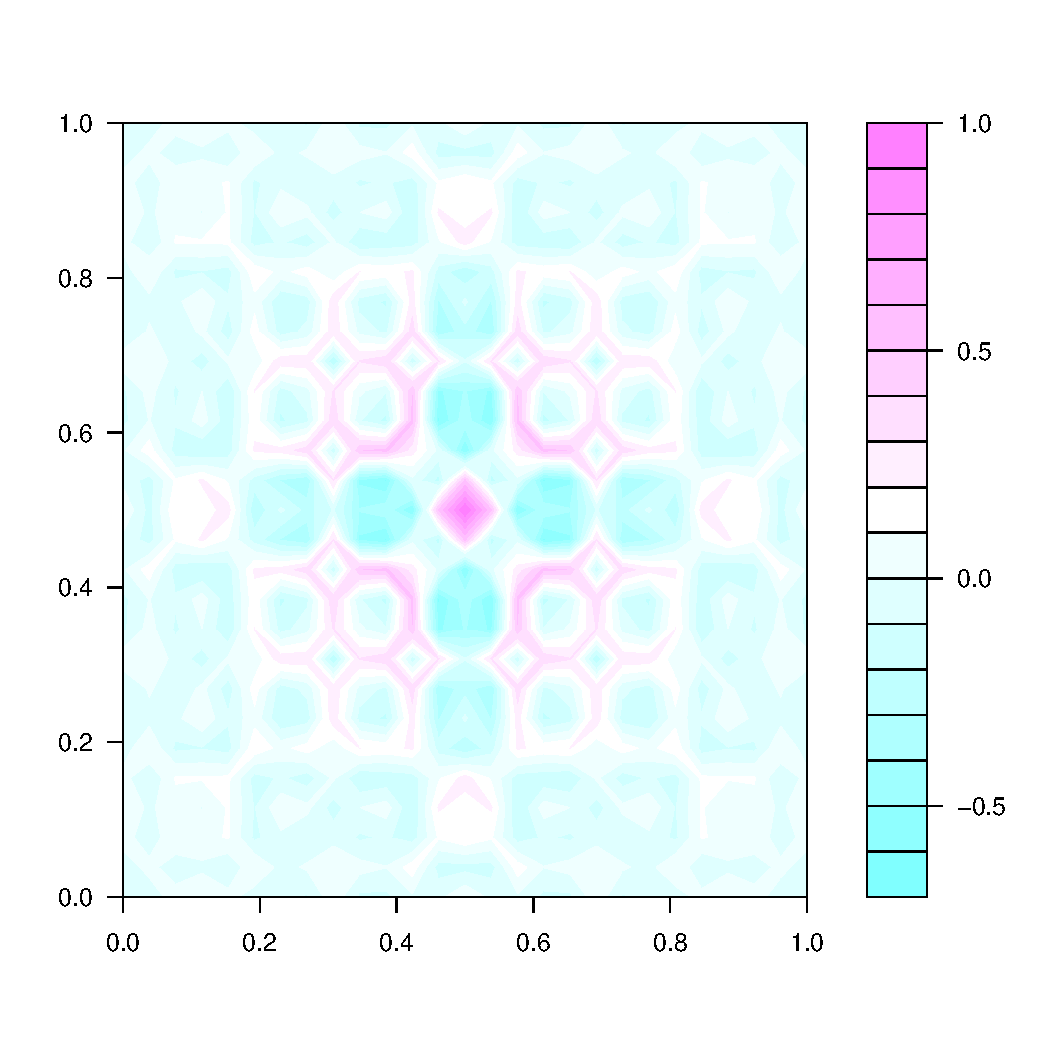
\includegraphics[height = 7cm, width = 7cm]{plot/filled_solution_2.pdf}
  \end{center}
}

\only<3>{
  Difference
  \begin{center}
  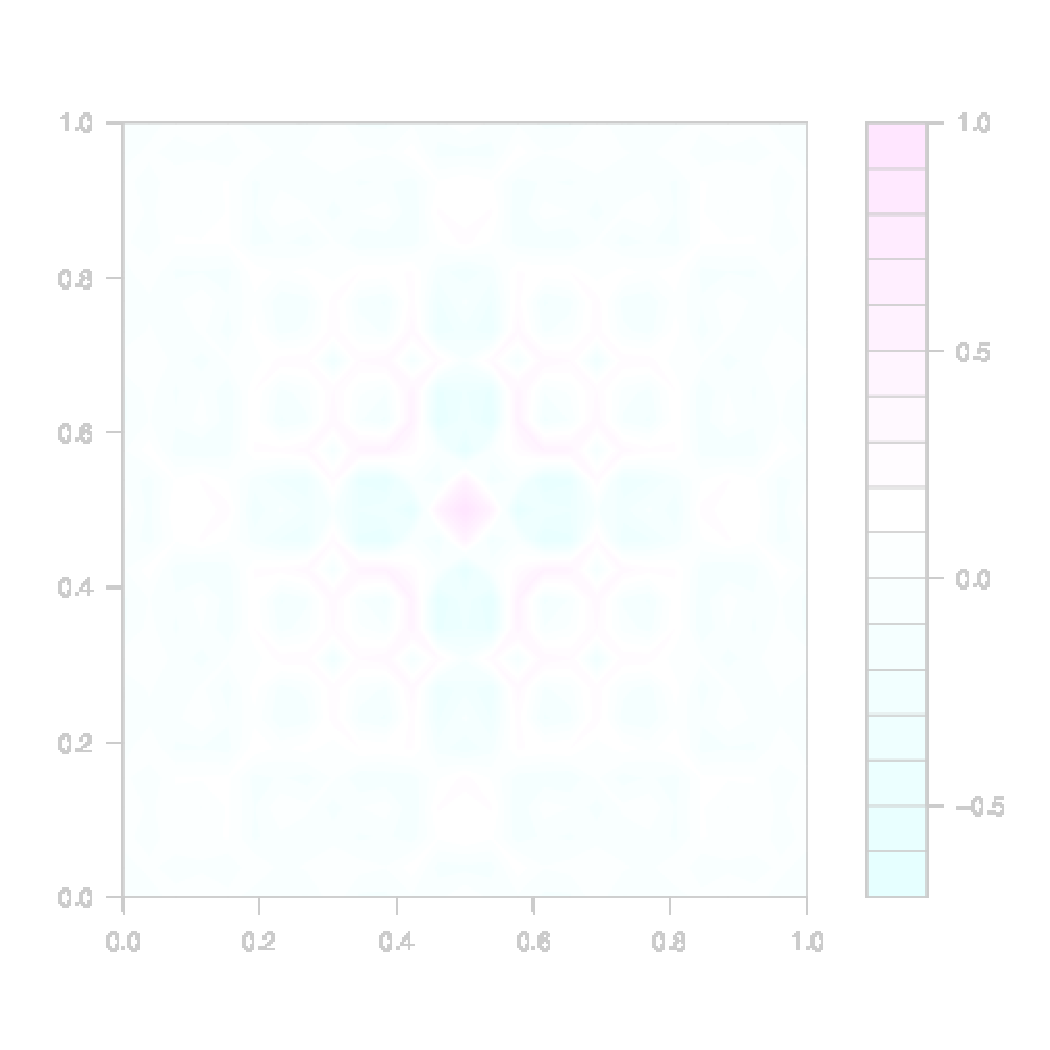
\includegraphics[height = 7cm, width = 7cm]{plot/filled_solution_diff.pdf}
  \end{center}
}


\end{frame}

%------------------------------------------------



\begin{frame}[fragile]
\frametitle{Why use \textbf{grid}?}

\only<1>{
  \texttt{> par(mfrow = c(1,2))}\\
  \texttt{> Volcano.persp()}\\
  \texttt{> box('outer', col = 'red')}\\
  \texttt{\textcolor{codegreen}{\#\# volcano\_filled.contour()}}\\

  \begin{center}
  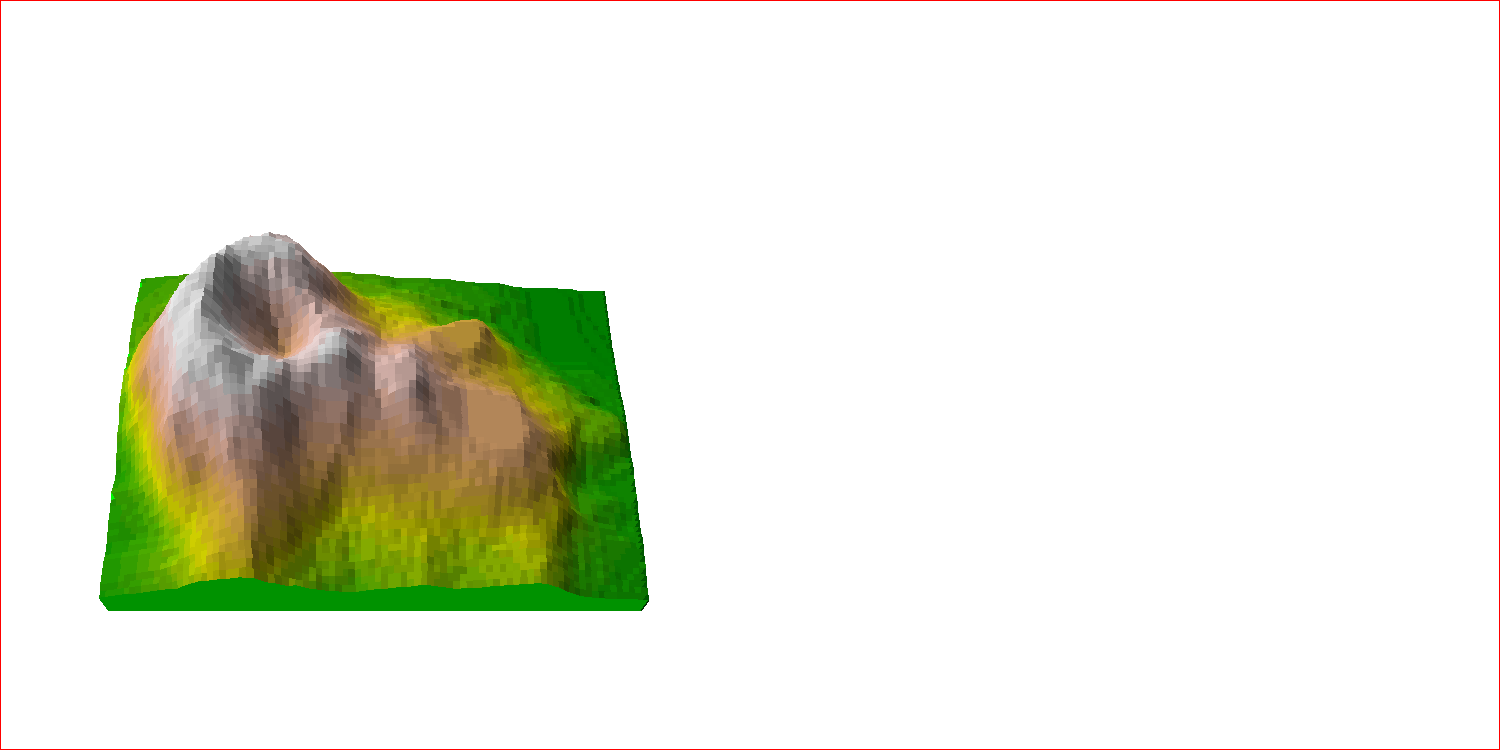
\includegraphics[height = 5cm, width = 10cm]{plot/demo_example_1.pdf}
  \end{center}
}

\only<2>{
  \texttt{> par(mfrow = c(1,2))}\\
  \texttt{> Volcano.persp()}\\
  \texttt{> box('outer', col = 'red')}\\
  \texttt{> volcano\_filled.contour()}\\
  \begin{center}
  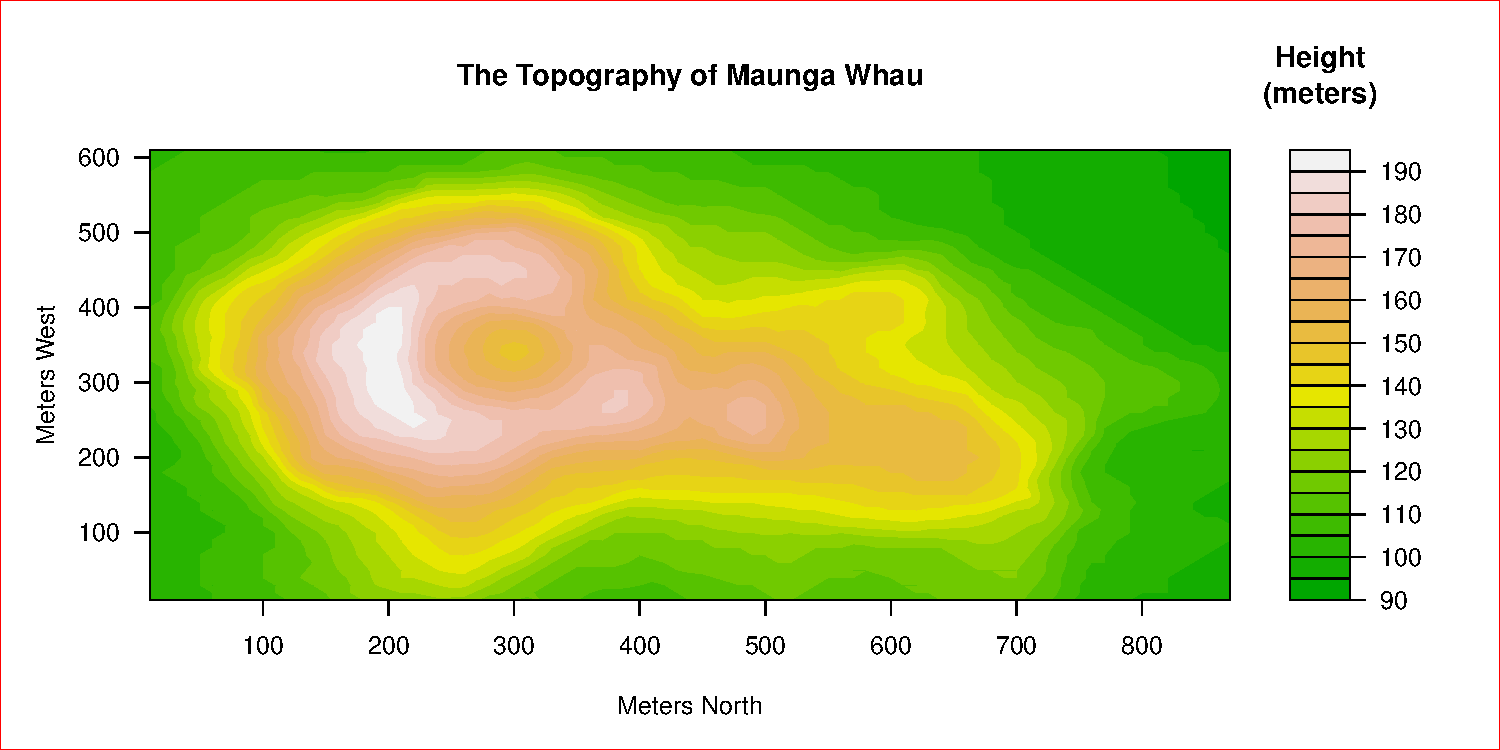
\includegraphics[height = 5cm, width = 10cm]{plot/demo_example_2.pdf}
  \end{center}
}

\end{frame}


\begin{frame}[fragile]
\frametitle{Why is \textbf{grid}?}

\begin{lstlisting}[language = R]
> vp = viewport(...)
> pushViewport(vp)
> grid.echo(Volcano.persp, newpage=FALSE)
> upViewport()
\end{lstlisting}

\begin{center}
  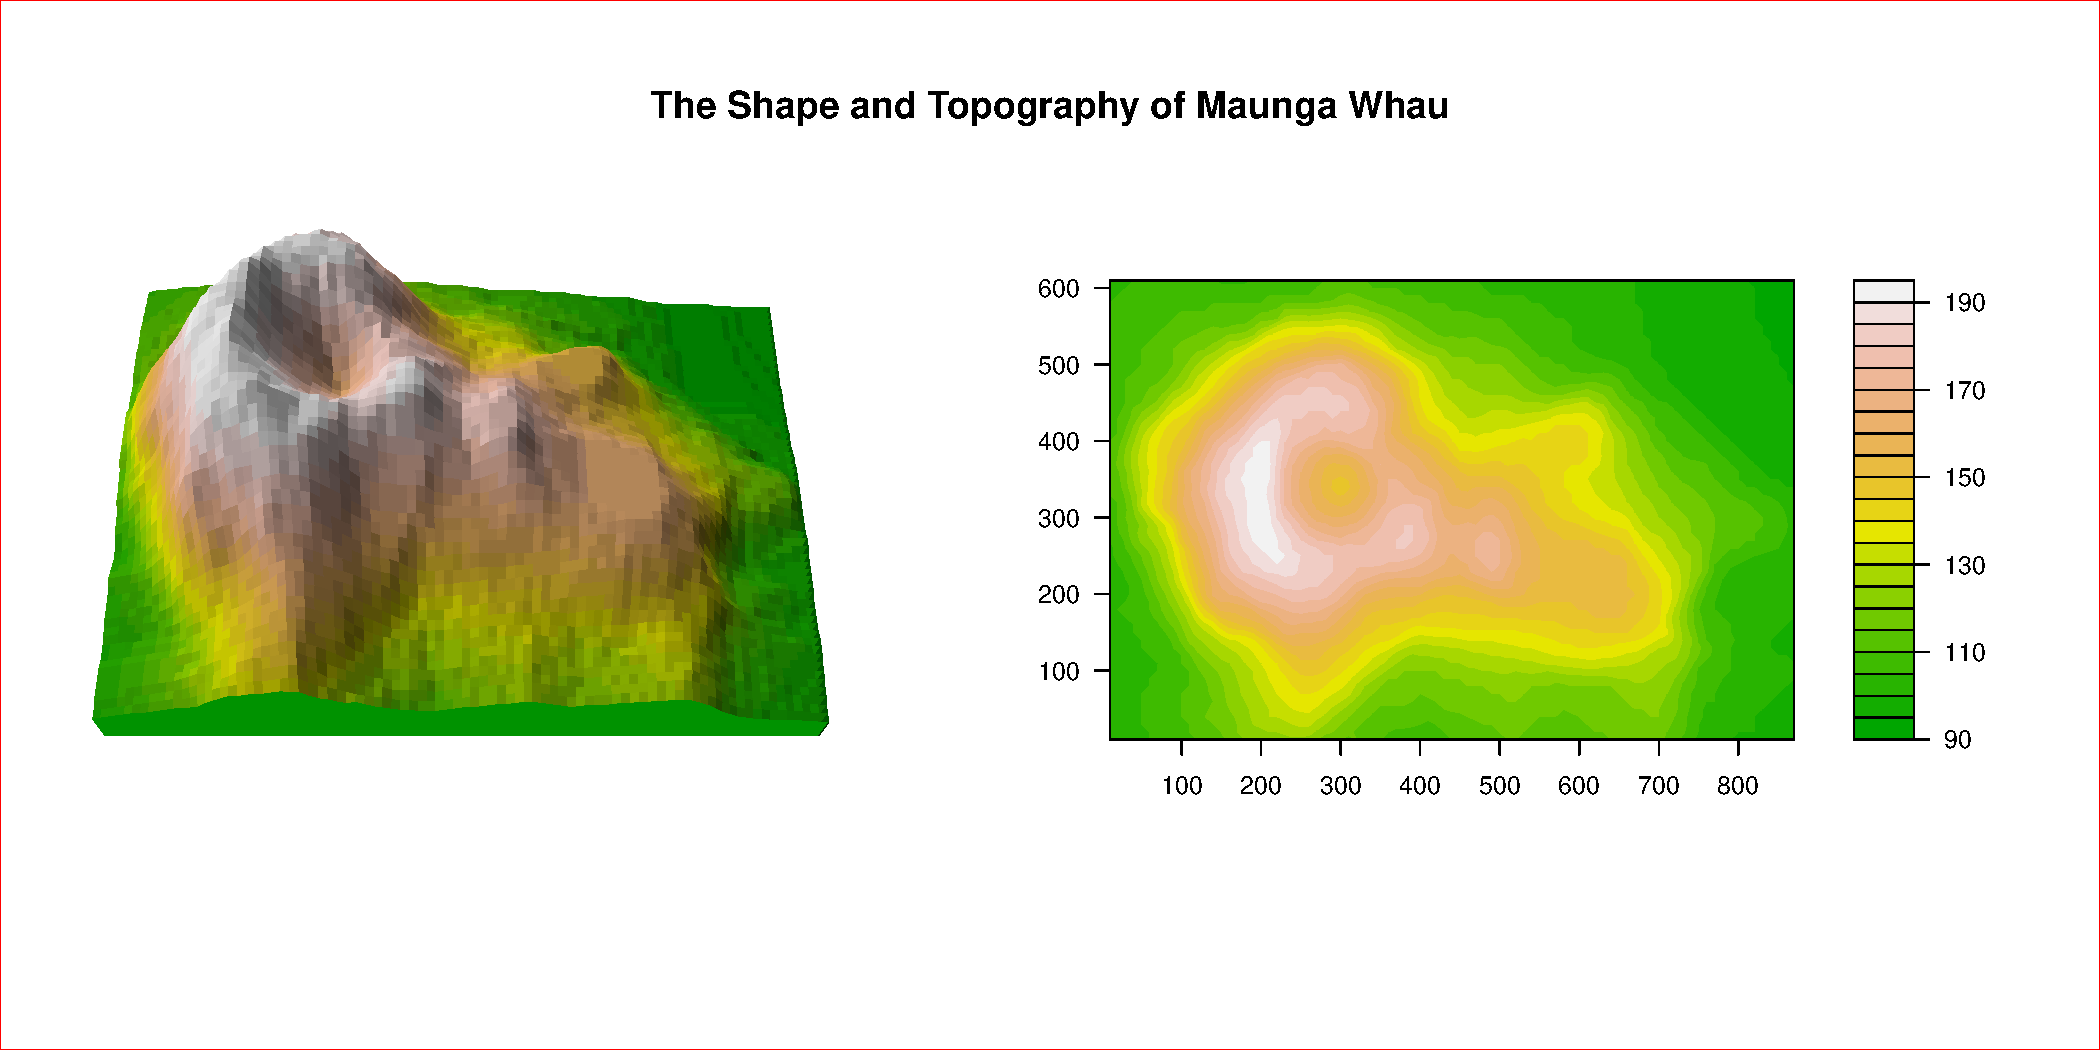
\includegraphics[height = 5cm, width = 10cm]{plot/demo_grid_example_3.pdf}
\end{center}

\end{frame}


\begin{frame}[fragile]
\frametitle{Why use \textbf{grid} (Advance)?}

\begin{lstlisting}[language = R]
> surface()
> addFeatures()
> grid.script(file = "example.js")
> grid.export("example.svg")

\end{lstlisting}

\begin{center}
  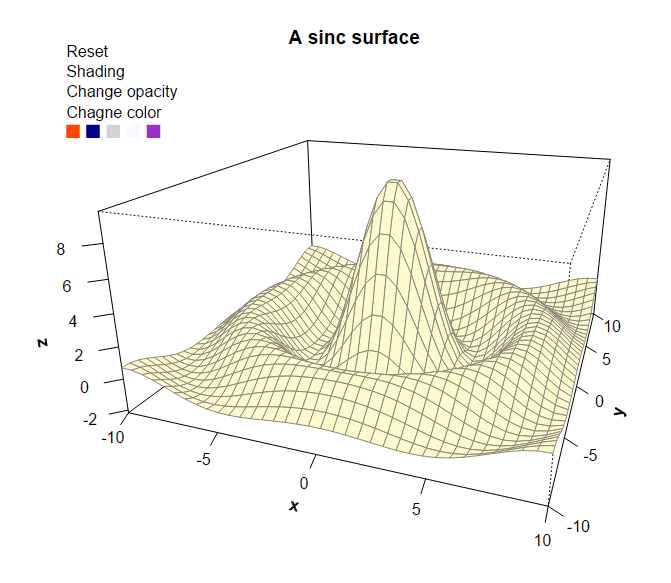
\includegraphics[height = 6cm, width = 7.5cm]{plot/origin_1.PNG}
\end{center}

\end{frame}


\begin{frame}[fragile]

\begin{center}
\Huge Any Question(s)?
\end{center}


\end{frame}





\end{document}
